\section{Methods}
\label{section:Methods}

\subsection{Fabrication}


\subsubsection{Electron Beam Lithography}
Fabrication of the junctions was done using electron beam lithography. This process is depicted schematically in figure \ref{fig:EBL}.
In this process, one starts with the substrate on which the device will be fabricated. The substrate used for all devices discussed in this thesis was p+ doped silicon covered by silicon oxide. The p+ doped silicon conducts electricity, while the silicon oxide is a dielectric. This means that the substrate can be used as a global back gate. This substrate is next cleaned using red fuming nitric acid.

\begin{figure}[H]
     \centering
     \begin{subfigure}[b]{0.49\textwidth}
         \centering
         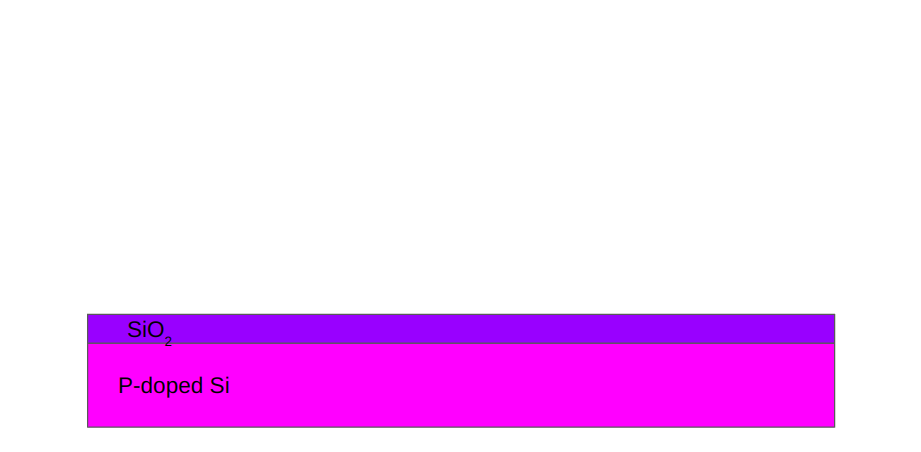
\includegraphics[width=\textwidth]{EBL1.png}
         \caption{A cleaned substrate.\newline}
         \label{subfig:EBL-a}
     \end{subfigure}
     \hfill
     \begin{subfigure}[b]{0.49\textwidth}
         \centering
         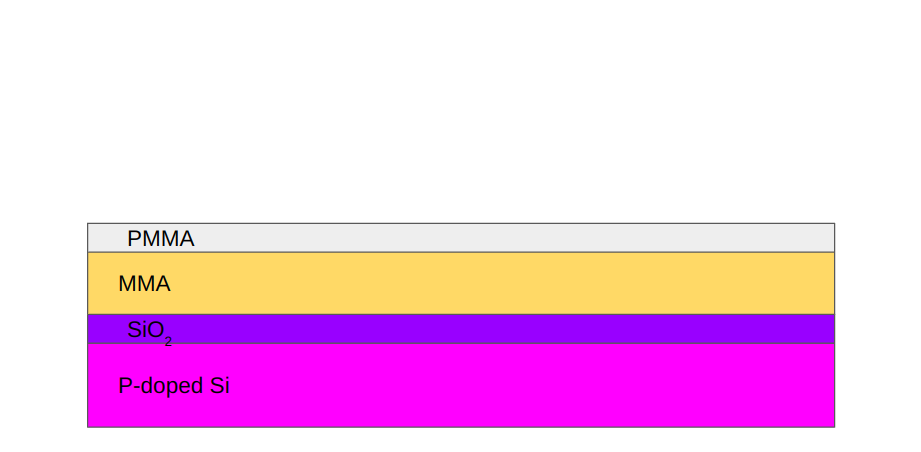
\includegraphics[width=\textwidth]{EBL2.png}
         \caption{Layers of PMMA and MMA are added onto the resist by spin-coating.}
         \label{subfig:EBL-b}
     \end{subfigure}
     \hfill
     \begin{subfigure}[b]{0.49\textwidth}
         \centering
         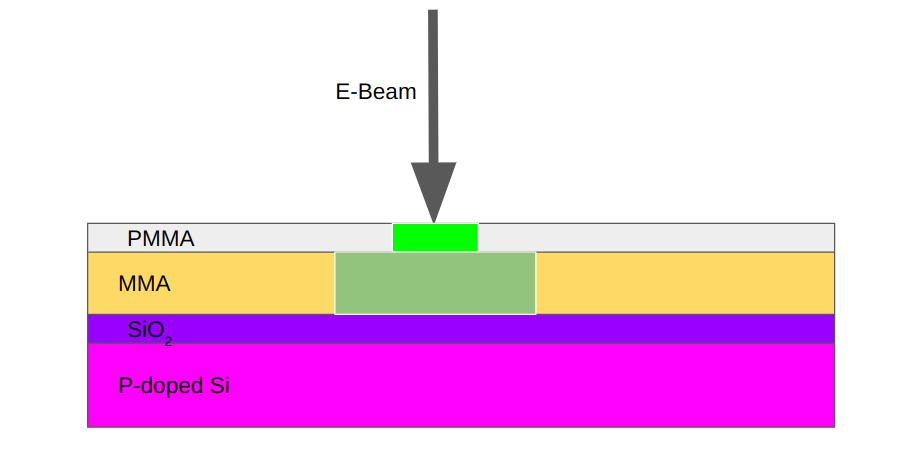
\includegraphics[width=\textwidth]{EBL3.png}
         \caption{A portion of the resist is irradiated with an electron beam in a specified pattern.}
         \label{subfig:EBL-c}
     \end{subfigure}
     \hfill
     \begin{subfigure}[b]{0.49\textwidth}
         \centering
         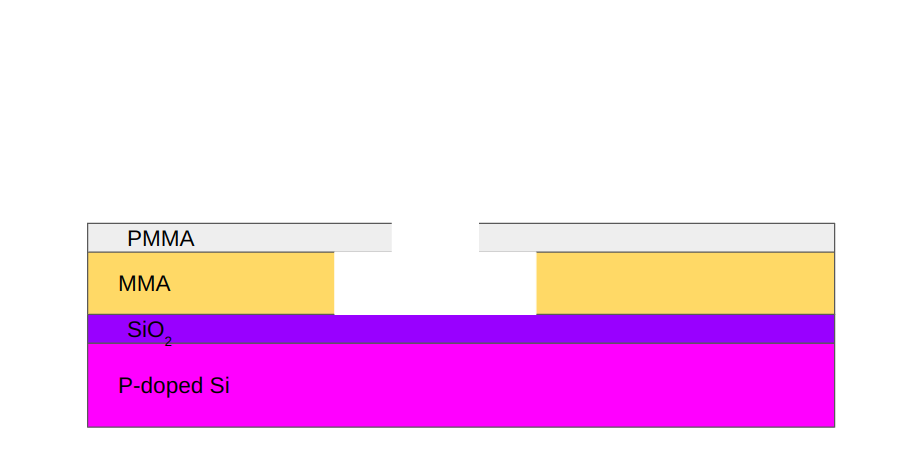
\includegraphics[width=\textwidth]{EBL4.png}
         \caption{The irradiated region is dissolved away. \newline}
         \label{subfig:EBL-d}
     \end{subfigure}
     \hfill
     \begin{subfigure}[b]{0.49\textwidth}
         \centering
         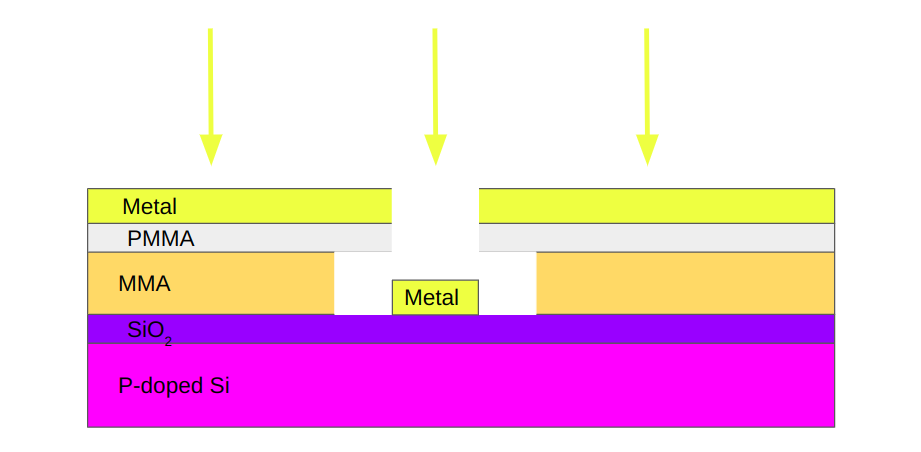
\includegraphics[width=\textwidth]{EBL5.png}
         \caption{Material is evaporated onto the mask and substrate.}
         \label{subfig:EBL-e}
     \end{subfigure}
     \hfill
     \begin{subfigure}[b]{0.49\textwidth}
         \centering
         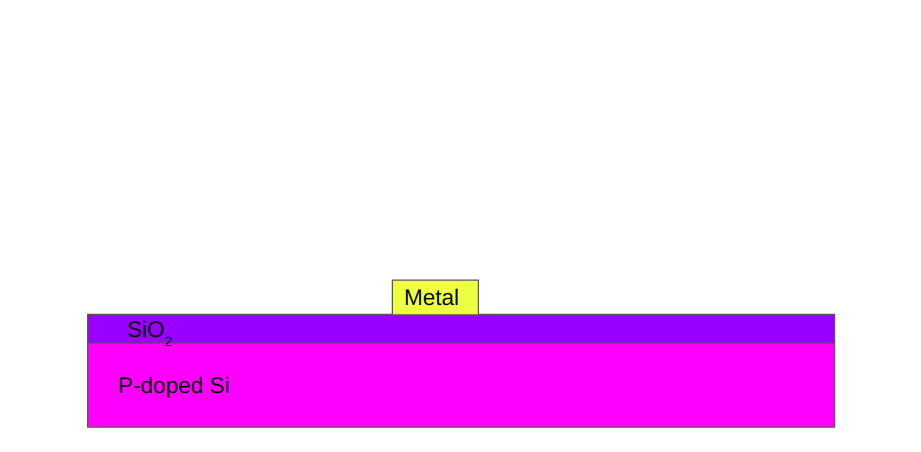
\includegraphics[width=\textwidth]{EBL6.png}
         \caption{The mask is removed, leaving the patterned material on the substrate.}
         \label{subfig:EBL-f}
     \end{subfigure}
        \caption{Electron Beam Lithography Process Diagram.}
        \label{fig:EBL}
        
\end{figure}

The cleaned substrate is covered by a layer of the resist methyl methacrylate (MMA),  which is dissolved in ethyl lactate at 8\% concentration, using a technique known as spin-coating. This technique allows for a very thin film of MMA to be deposited, with a high level of control on the final thickness. The MMA was spin coated at 2000 rpm for one minute and next baked for 5 minutes at 180 $^{\circ}$C to remove the solvent and fix the resist. This recipe creates an MMA layer of 340 nm thick. On top of this layer, 80 nanometers of poly methyl methacrylate (PMMA) with a molecular weight of 950K, dissolved in anisole at 2\% concentration, is deposited by spin coating for 60 seconds at 2000 rpm, which is also followed by a 5-minute bake at 180 $^{\circ}$C, which creates a layer of PMMA of 80 nm thick (Figure \ref{subfig:EBL-b}).

PMMA and MMA are both sensitive to electron bombardment. When these resists are irradiated with electrons, polymeric chains are broken and as a result the solubility is increased (Figure \ref{subfig:EBL-c}, color change reflects change in solubility). An electron beam lithography machine is able to expose the resist in a specified pattern with a resolution of close to 1 nm. Due to the additional exposure of the resist by indirect, scattered electrons, the maximal resolution is reduced to the order of 10 nanometers. Due to the lower molecular weight of the MMA compared to the PMMA, the MMA needs less exposure to become soluble. This causes a larger region of MMA to be effectively irradiated.

After exposure with the electron beam, the sample is developed by submersing it in a 3 to 1 mixture of isopropyl alcohol (IPA) to methyl isobutyl ketone (MIBK) for 90 seconds. This causes the exposed area of the resist to dissolve and be removed, while the less soluble unexposed resist remains (Figure \ref{subfig:EBL-d}). Since a larger area of PMMA was effectively exposed compared to the MMA, there is a region where the PMMA gets removed while the apposed MMA remains. This region of the PMMA is called the undercut, while the region of MMA that hangs above the undercut is called an overhang. The sample is next transferred to pure IPA to stop the development process. After development, the sample is exposed to oxygen plasma for 20 seconds. This is a cleaning step that removes unwanted residues that may have been left after the development.

Next, the mask that was created in the preceding steps is ready for metallization. It is placed in an evaporation chamber, and metal is deposited using electron beam evaporation. This results in a thin layer of metal being deposited on the sample, as shown in figure \ref{subfig:EBL-e}. Many metals do not stick to the SiO$_2$ layer reliably, and as a result they may come off during further fabrication steps. To remedy this, often a different layer of metal is deposited on the SiO$_2$ first. Such a layer is known as a sticking layer, and all devices discussed in this thesis have been made using a 5 nm titanium sticking layer.

Finally, the mask and the portion of the metals that was deposited on top of the mask is removed, in a process known as lift-off. This is done by submersing the sample in N-Methyl-2-pyrrolidone (NMP), heated to 80 $^{\circ}$C for multiple hours. This dissolves the resist and thereby also removes the metal that was supported by that resist, as shown schematically in figure \ref{subfig:EBL-f}.

\subsubsection{Double Angle Evaporation}
In the preceding subsection an outline of the EBL process was described. If one wants to design a device with multiple layers of metal, where each metal is deposited in a different shape, the entire EBL process can be repeated. The resist is applied on top of the substrate and the already deposited metal, and irradiated according to a new pattern. After development this will form a new mask such that a new layer of metal can be evaporated onto the substrate in a different pattern. A notable difficulty with this method of producing different patterned layers is that the patterns of the different layers need to be properly aligned. This alignment happens with finite accuracy, and therefore can introduce imperfections in the device geometry. Another drawback is that it is more arduous to go through all the EBL steps a second time than it would be to reuse the same mask for multiple layers. 

\begin{figure}[H]
     
     \begin{subfigure}[b]{0.49\textwidth}
         \centering
         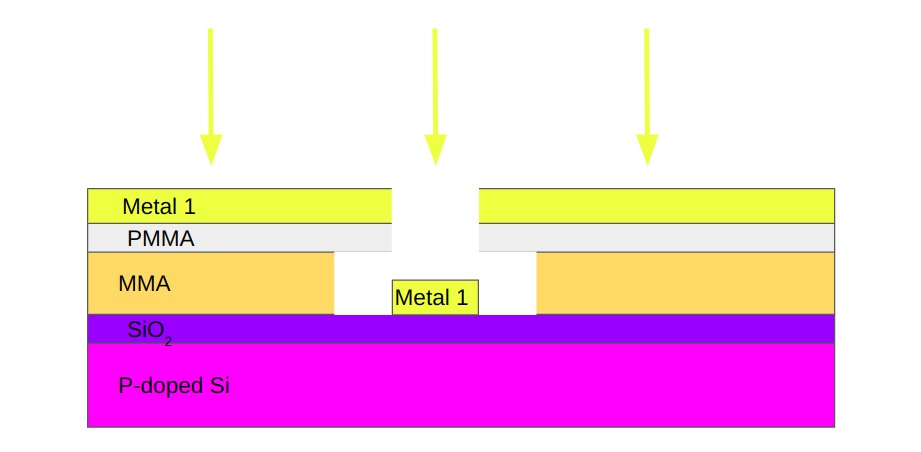
\includegraphics[width=\textwidth]{DoubleAngle1.png}
         \caption{The first layer of material is evaporated onto the mask and substrate. \newline}
         \label{subfig:evaporation-first}
     \end{subfigure}
     \hfill
     \begin{subfigure}[b]{0.49\textwidth}
         \centering
         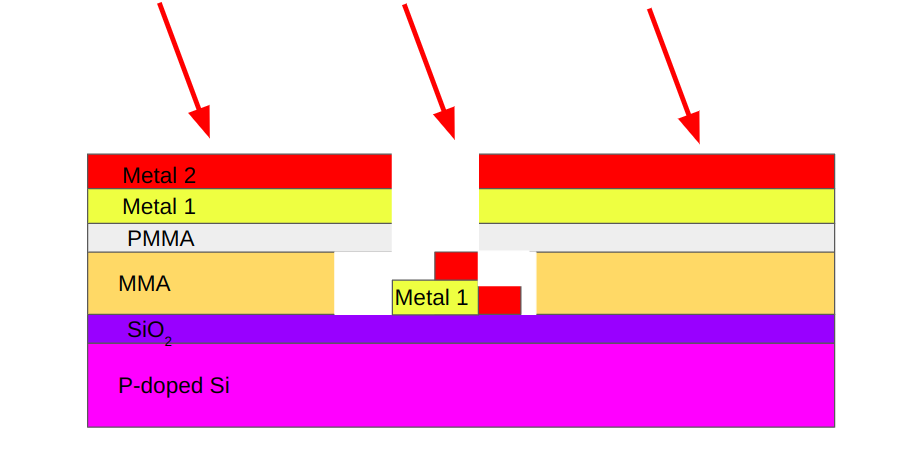
\includegraphics[width=\textwidth]{DoubleAngle2.png}
         \caption{The second layer is evaporated at a different angle, causing a translation with respect to the first layer.}
         \label{subfig:evaporation-second}
     \end{subfigure}
        \caption{Double angle evaporation.}
        \label{fig:DoubleAngle}
        
\end{figure}

There is another way of creating a device with multiple differently patterned shapes that only involves the use of a single mask. This process is known as double angle evaporation. As the name suggests, double angle evaporation involves evaporating the different layers of metal at different angles. Since the mask has a nonzero thickness, the different angles result in a relative translation between the different evaporated layers. Evaporating the material at an angle with respect to the normal of the substrate also causes a stretching of the masked pattern. Because the same mask is used for different layers of material, these layers are automatically well aligned. There are some drawbacks to this method. One drawback is that the different layers need to be translated copies of each other, making this technique only useful in cases where this class of patterns is sufficient for the device being fabricated. Another drawback is that whenever material is evaporated at an angle to the normal, there needs to be enough undercut to accommodate the translated pattern. When undercuts get too big, the corresponding overhangs can become unstable and the mask may fail. 

\subsubsection{Design}

Most often, when contacting nanoscopic objects using EMBJs, the bridge material of choice is gold. Gold atoms have a relatively high mobility, which makes electromigrating gold easier and allows for self breaking at room temperature. Gold is also highly unreactive, such that the quality of the contacts is not degraded by oxidation as it would be with a more reactive material. Another reason to choose gold is that it has a relatively high electrical conductance. The most obvious drawback, however, is that not all objects can be optimally contacted with gold. Some objects, such as GNRs, have a work function that does not match as well with the work function of gold as with some other metals, which can result in Schottky barriers or poor band alignment. For those objects, a different bridge material needs to be chosen. Palladium has been found to have a work function that is well suited for contacting GNRs [9], and even more so for contacting carbon nanotubes. Palladium atoms are less mobile than those of gold, which means that migration may require larger temperatures or currents, and that self-breaking at room temperature does not typically take place, or takes place only over much larger time scales. Palladium is also slightly more reactive than gold. For many objects that are hard to contact with gold, and GNRs specifically, palladium is a good choice for the bridge material. This is why palladium was chosen as the bridge material to be studied in this thesis.\\


\noindent Since the goal is to create superconducting EMBJs, and since palladium does not by itself become superconducting at low temperatures, superconductivity needs to be induced in the palladium using the proximity effect. 

From our discussion on the proximity effect in the chapter on Theory, specifically equation \ref{eq:BilayerTc}, we conclude that the best way to induce superconductivity in the palladium is by having a thin palladium layer covered by a thick layer of superconductor, at least in the limit where both films are much smaller than their respective coherence length. The superconductor should have a high $T_C$ and a high DOS at the Fermi energy. Niobium was chosen in the designs studied in this thesis, since out of the available superconductors it has a good combination of a high $T_C$ with a relatively high DOS at the Fermi level. The fact that niobium can be evaporated means that double angle evaporation is possible, since the deposition is unidirectional when depositing using evaporation. When depositing material using sputtering, however, deposition happens in all directions making double angle evaporation impossible. As mentioned, using double angle evaporation makes the fabrication process significantly easy and less susceptible to error by eliminating the need for multiple cycles of spin coating, e-beam and development, and the need to align successive patterns.\\


\noindent Having selected palladium for the bridge material and niobium for the proximitizing superconductor, and single step double angle evaporation for the fabrication, we need to determine the geometry of the devices. The main geometric choices to be made are the respective thicknesses of the palladium and niobium, the distance between the niobium and the center of the bridge and the constriction geometry.

For the constriction geometry, the main design goals are to reliably have electromigration create the gap in the center of the bridge, and to have a high electronic diffusion coefficient throughout the bridge, since that implies a higher Thouless energy

When electromigration consistently happens near the center of the bridge, the chance that other materials than the bridge material, such as the titanium sticking layer or the niobium layer, diffuse into the leads during electromigration. Such a mixing of different kinds of atoms leads to reduced diffusion and thereby reduced superconductivity, and it leads to an uncontrolled and undesired contact surface. Consistency in breaking is furthermore desirable since a variable gap location, which leads to variable superconducting properties, adds an uncontrolled variable to transport measurements done using the EMBJ and reduces interpretability and reproducibility of the results. Electromigration is most likely to start in areas of high local resistance, and is especially likely to start at grain boundaries. Since the local resistance of the bridge is inversely proportional to the local cross-sectional area, a sharp constriction where the cross-sectional area is much smaller in the center than in the rest of the bridge will most reliably break close to the center. 

Since the Thouless energy is proportional to the electronic diffusion coefficient in the bridge, we want to choose a geometry in which this coefficient is high. The electronic diffusion coefficient is proportional to the electron mean free path. In thin films, such as our bridge, the effect of edge scattering on the mean free path is significant. In a very constricted geometry, the mean free path becomes very small near the constriction due to edge scattering, and diffusion becomes poor. 

\begin{figure}[H]
     
     \begin{subfigure}[b]{0.49\textwidth}
         \centering
         
\includegraphics[width=\textwidth]{restriction_tight.png}
         \caption{A sharp constriction, with good gap localization but poor diffusion.}
         \label{subfig:constriction-sharp}
     \end{subfigure}
     \hfill
     \begin{subfigure}[b]{0.49\textwidth}
         \centering
         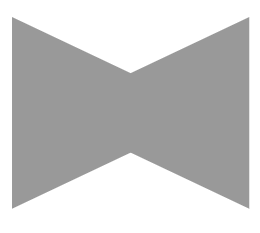
\includegraphics[width=\textwidth]{restriction_loose.png}
         \caption{A blunt constriction, with good diffusion but poor gap localization.}
         \label{subfig:constriction-blunt}
     \end{subfigure}
        \caption{A comparison of restriction geometries.}
        \label{fig:ConstrictionGeometries}
        
\end{figure}

In our design, a bowtie geometry with a 60$^\circ$ constriction angle was chosen because it was hypothesized to be a good compromise between having good diffusion and good gap localization.\\


\noindent The choice of palladium thickness is motivated by our desire to have good induced superconductivity and good electromigration.

In order to have good electromigration, the bridge resistance should be high compared to the series resistance. Since the bridge resistance is smaller for thicker bridges, the bridge thickness should not be so big that electromigration becomes difficult. 

In order to have good superconductivity, there are two competing considerations. Equation \ref{eq:BilayerTc} tells us that the palladium will have a higher induced $T_C$ when it is thinner compared to the niobium, at least in the thin film limit. A thicker palladium layer also causes more inverse proximity effect in the niobium, thereby increasing the effective distance from the niobium to the gap. It also reduces the energy gap in the bilayer.

The mean free path of the leads, on the other hand, is inversely proportional to the resistivity of the film, which increases with thinner films. This therefore leads to a reduced Thouless energy. 

Based on these considerations, a palladium thickness was chosen to be 13 nm in the bridge.\\

\noindent Based on the theoretical discussion of the proximity effect, we concluded that a thicker layer of superconductor implies a better proximity effect, where the proximity effect starts to saturate asymptotically as the thickness of the superconductor becomes much larger than the coherence length of the superconductor. Therefore, we wish to make the niobium layer as thick as possible within the constraints of the fabrication process. 

Niobium has a very high evaporation temperature. Consequently, the substrate on which the niobium is deposited is heated substantially during the deposition. When more niobium is deposited, more heating takes place and more film stress can develop. This can damage the resist layer and lead to fabrication defects. Thinner layers tend to have a cleaner fabrication with fewer defects. 

Based on these considerations, our initial guess for the ideal thickness of the niobium layer was 100 nm.\\


\noindent The degree of proximitization of the normal metal decreases as the distance to the superconductor increases. In order for the leads to be optimally proximitized the niobium should be deposited as close to the center of the bridge as possible without any niobium ending up at the site where the break is created during electromigration. When using shadow mask evaporation, there is always a region around the pattern where small amounts of material inadvertently end up. If the niobium layer is patterned too close to the center of the bridge, this will lead to unintended niobium deposition onto the leads. This constrains the distance between the niobium deposition region and the center of the bridge. In our design, we chose this distance to be 25 nm. \\


\noindent As mentioned in the section on EBL, a 5 nm titanium sticking layer is used to ensure that the other layers stick to the substrate. The sticking layer is evaporated at a right angle to the substrate, such that it does not end up underneath the bridge. Since the bridge has only a small contact area with the surface, its connection to the rest of the device is sufficiently strong to hold it in place and no sticking layer is needed there. The absence of titanium under the bridge reduces the likelihood of a palladium titanium alloy forming during the migration process. This increases the probability that the resulting contacts are made of pure palladium as intended. The absence of titanium under the bridge also improves the superconductivity of the bridge, since titanium is a normal metal above 0.49 K and would inversely proximitize the bridge in that temperature range. The final device design is depicted in figure \ref{fig:device_design}.

\begin{figure}[H]
     \centering
     \begin{subfigure}{\textwidth}
         \centering
         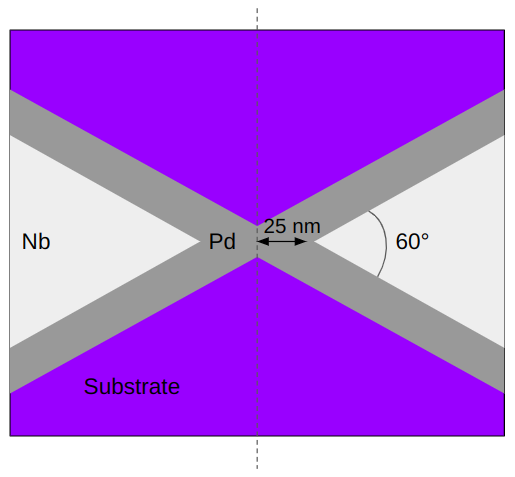
\includegraphics[width=0.6\textwidth]{layout_top.png}
         \caption{Device design, top view. The titanium sticking layer is located underneath the palladium, in the same pattern as the niobium.}
         %\label{}
     \end{subfigure}
     \newline
     \begin{subfigure}{\textwidth}
         \centering
         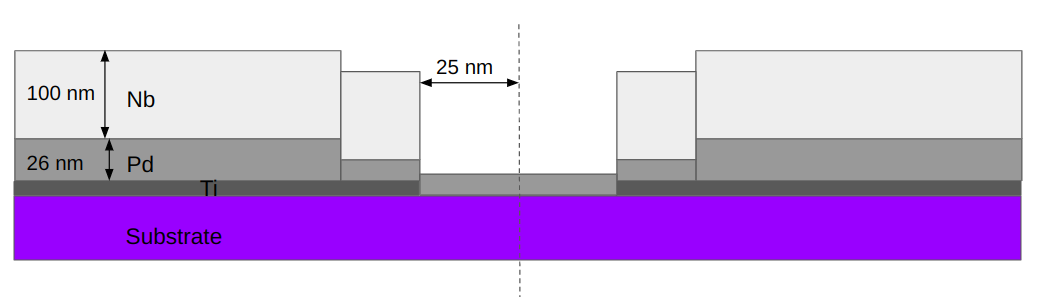
\includegraphics[width=\textwidth]{Layout_Side_2.png}
         \caption{Device design, side view.}
         %\label{}
     \end{subfigure}
        \caption{Device design.}
        \label{fig:device_design}
        
\end{figure}

\subsubsection{Further Design Iterations}
During this thesis, the initial design outlined in the previous section was iteratively changed a total of three times. The goal in each design iteration was to improve the electromigration and superconducting qualities of the device. The changes that were made were in each iteration were based on the information gained from the results of transport measurements that were done on the devices of the previous iteration. In some cases the changes were also based on the results of fabrication tests. Devices made with the initial design are referred to in this thesis as PdNb devices.  

The first change that was made was the substitution of gold for palladium as the bridge material. This change was made because no superconductivity was measured in the PdNb devices after electromigration. Since gold has a density of states at the Fermi energy that is approximately an order of magnitude lower than that of palladium, this substitution was hypothesized to increase the degree to which the bridge material was proximitized. Devices made with this second design are referred to in this thesis as AuNb devices, or sometimes AuNb devices with 100 nm niobium thickness.

In the second design iteration the thickness of the niobium layer was reduced from 100 nm to 50 nm, and the thickness of the gold layer was increased from 13 nm in the bridge to 15 nm. The rate at which the niobium was evaporated was also increased, from 0.2 nm/s to 0.5 nm/s. The reason for decreasing the thickness of the niobium layer and increasing its evaporation rate was that SEM images of the devices with the previous design showed that the niobium layer was not shaped as intended, while niobium layers evaporated with the new parameters were shown to be as intended in a fabrication test. The motivation for increasing the gold thickness was that a thicker layer of gold has a larger conductance and therefore a larger mean free electron path and a higher electronic diffusion constant, which leads to better proximitization of the bridge and an increase in the Thouless energy. The downsides of a thicker layer of gold is a lower bilayer $T_C$, and a lower bridge resistance, which is disadvantageous to electromigration. Despite this trade-off, it was hypothesized that a thicker gold layer would improve device quality. The devices made with this design are referred to in this thesis as AuNb devices with 50 nm Nb.

The final design change was an increase in the bridge length from 50 nm to 60 nm. It was hypothesized that this change would lead to more consistent gap formation during electromigration. Devices with this design are referred to in this thesis as AuNb devices with 60 nm bridge spacing. 

\subsubsection{Chip Preparation}

Devices were typically fabricated on a 19 mm by 19 mm substrate, with a layout as shown in figure \ref{fig:device_layout}. On this substrate, a grid of 9 sets of devices was usually fabricated, where each set contains 5 rows of 8 devices.

\begin{figure}[H]
     \centering
     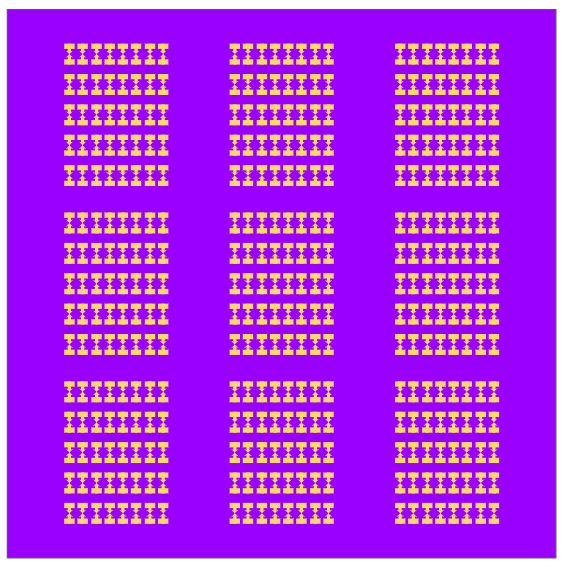
\includegraphics[width=0.6\textwidth]{device_layout.png}
     \caption{A schematic representation of the final device layout on the substrate.}
     \label{fig:device_layout}
        
\end{figure}

In order to be able to load the devices into the measurement set-up, they need to be put on a chip carrier. Because of the size of the chip carrier, the 19 mm by 19 mm substrate needs to be cut into 9 separate pieces, each containing a single set of devices. One such set then fits on the chip carrier. The substrate was first scratched using a diamond tipped scratcher along a crystallographic direction and then broken along this scratch by applying a bending force to the substrate using breaking pliers. The set of devices thus obtained is then attached to the chip carrier using either silver paste or two-sided carbon tape. Both silver paste and carbon tape are electrically conducting, which creates an electrical connection between the backplate of the chip carrier and the doped silicon of the substrate. Finally, the devices are connected to the chip carrier. The chip carrier contains pads made for electrical connections, and each device has two bonding pads for the same reason. Using a device called a wirebonder, small aluminium wires can be made between the pads of the chip carrier and the bonding pads of the devices. One connection is made between a pad of the carrier and the backplate of the carrier. This pad will allow a gate voltage to be applied to the devices. At this point, the device is ready to be loaded into the measurement set-up. The chip carrier containing a chip and wirebonds, connected to the backplate via silver paste, is shown in figure \ref{fig:chip_carrier}.

\begin{figure}[H]
     \centering
     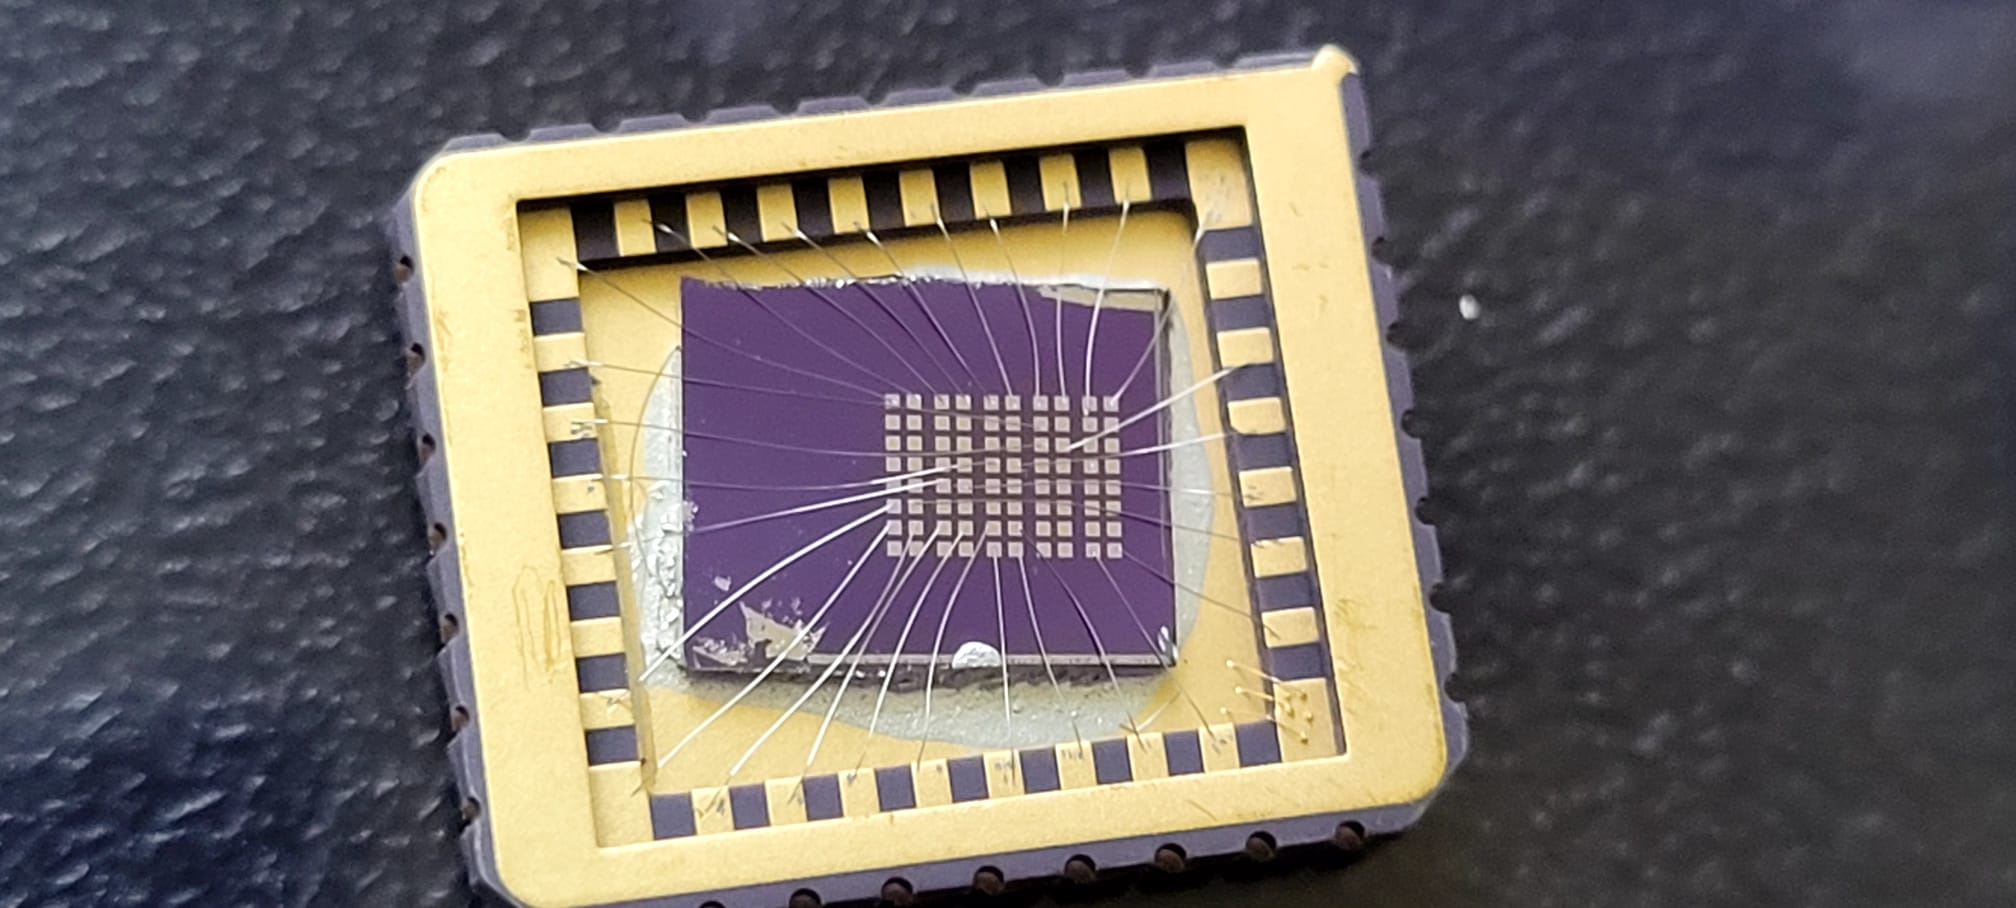
\includegraphics[width=\textwidth]{chip_carrier.jpeg}
     \caption{A chip carrier containing a substrate with a single set of devices. The substrate is connected to the backplate via silver paste. The bonding pads of the devices are connected to the pads of the chip carrier via aluminium wire bonds. A single pad of the chip carrier is connected via wirebonds to the backplate (bottom right).}
     \label{fig:chip_carrier}
        
\end{figure}


\subsection{Transport Measurements}
\label{subsection:transport_measurements}

Since the devices have been designed to break as a result of an applied voltage, electrostatic discharge (ESD), which can supply a sudden pulse of hundreds of volts, can easily destroy a device. Because of this, care needs to be taken to ensure that the devices are protected from ESD. The way this is done is by always wearing a grounding bracelet while touching any modules that are connected to the device, and keeping the devices themselves grounded while measurements are not being performed on them.\\

In order to reach the temperatures needed to observe the superconducting effects of interest at high enough resolution, two cooling setups were used. Both involve the use of liquid helium. Liquid helium has a boiling point of around 4.2 K at atmospheric pressure. 

In the first setup, the sample is loaded into a stick, the so-called dip stick. The interior of the stick contains an inner vacuum chamber where the sample is placed, which is separated from the outside, and a second smaller chamber called the 1K pot, which is connected to the outside of the stick by a small opening which can be opened or (partially) covered using a valve by the operator. The sample makes thermal contact with the 1K pot. The pressure in the main chamber and in the 1K pot can be controlled by attaching pumps to the stick. This stick is submerged in a dewar of liquid helium. By creating a small opening between the 1K pot and the liquid helium while pumping the 1K pot, helium is let into the 1K pot but the pressure inside will be lower than atmospheric pressure. This results in a lowered boiling for the helium and reduces the sample temperature, theoretically as low as 1 K but in practice in this set-up a minimal temperature of 1.6 K was more typically reached. The dipstick set-up contains a heater which allows the temperature to be raised and temperature dependent measurements to be performed. The dipstick set-up contains no magnet and thus no magnetic field dependence can be measured.

The second measurement set up involves a dilution fridge. The dilution fridge is a machine that uses the mixing of two helium isotopes, He$^3$ and He$^4$, to reach temperatures as low as 25 mK. The dilution fridge also contains a vector magnet, which allows the operator to apply a magnetic field in any direction. The magnetic field has a maximum magnitude which depends on direction. In the direction perpendicular to the chip, which we will henceforth refer to as the Z direction, the magnetic field can go as high as 10 T. In the two perpendicular directions which are in plane with the chip, referred to as the X and Y directions, the magnetic field can reach 1 T and 3 T respectively. The presence of the vector magnet allows for measurements with magnetic field dependence in this set-up, and the lower temperatures that can be reached allow for higher resolution measurements.\\

In each of the measurement setups, there is a holder that the chip carrier can be loaded into. This holder contains pins that connect the pads of the chip carrier to a different set of pins which allow the operator to connect to the devices during the measurements. The module containing these pins is called the matrix module, and the rack that this module and the other modules used during a measurement are placed in is called the IVVI-rack. By connecting modules that apply or measure current or voltage to the pins of the matrix module, the operator can perform transport measurements. \\

When doing a transport measurement, care needs to be taken with the choice of measurement to ensure that the measurement is of high quality. In order to ensure this, the operator must choose modules that optimize the input impedance of the measurement modules and the output impedance of the source modules, as well as the amount of noise that results in the measurement. Series resistance and noise lower the quality of the measurement because they result in systematic and random error, respectively. Since the setup is controlled digitally, care must be taken to minimize the influence of the finite precision digital values sent to the IVVI rack.\\

\subsubsection{VI}
One of the most elementary measurements is one where a current source applies a bias current to the device, and voltage is measured over the device. I will refer to this kind of measurement as a VI measurement. With such a measurement, the instructions on what bias to apply are sent to the IVVI rack from the computer. The IVVI rack converts this digital signal to an analog one using a digital to analog converter (DAC). This results in a voltage of between -1.5 V and 1.5 V that is supplied to the current source module. The current source module has a built-in amplifier with multiple possible configurations ranging from 1 nA/V to 10 mA/V, which determines the amount of current it delivers per unit of voltage supplied by the DAC. The amplification setting also determines the output resistance of the module. The output resistance is one over the amplification, such that at 1 nA/V the output impedance is 1 G$\Omega$ and at 1 mA/V it is 1 k$\Omega$, for example. The current is biased over a device, using the appropriate pins from the matrix module. The voltage measurement module is applied in parallel over the same device. This creates a quasi 4 point measurement. The voltage measurement module has an amplifier that can be set to an amplification ranging from 1 to 10k. This module also has a maximal output voltage of 1.5 V. The output of the voltage measurement module goes to a Keithley-2100 digital multimeter, and the value that is measured there is stored on the computer. In order to minimize the digitization error introduced by the limited digital precision, the maximal range of the DAC should be used. For a current source, higher output resistance improves measurement accuracy and therefore the lowest possible amplification should be used. The largest possible amplification should be applied on the voltage measure module that allows it to stay below the maximal voltage, in order to make the most accurate use of the multimeter. 

Compared with a measurement where voltage is biased and current measured, a VI measurement introduces low series resistance and is therefore the appropriate choice when measuring a low resistance device. In this thesis all devices with a resistance less than one quantum of resistance were measured using the VI setup.\\ 




\subsubsection{IV}

When the resistance of the device to be measured is greater than one resistance quantum, we bias voltage and measure the resulting current. I will refer to such a measurement as an IV measurement. At high resistances, IV measurements allow for higher precision.

In the setup for an IV measurement, the voltage source, device and current measurement module are set up in series. The voltage source module receives the signal coming from the computer via the DAC and amplifies it, with an amplification of either 100 uV/V, 1 mV/V, 10 mV/V or 100 mV/V. These amplification settings have corresponding input resistances of 1 $\Omega$, 10 $\Omega$, 100 $\Omega$ and 1k $\Omega$ respectively. To achieve the lowest possible source resistance, the lowest possible amplification should be used.


The current measurement module again has an amplifier built in which determines how much voltage it outputs per measured unit of voltage, with an amplification ranging from $10^6$ to $10^9$ times. The input resistance again depends on the amplification, now as R$_{in}$ = 2k$\Omega$ + amplification/1000. The current measure amplification should set high enough that the signal-to-noise ratio is good but not so high that the input resistance is significant with respect to the device resistance, i.e. more than 1 percent.\\


\subsubsection{VIT / IVT, BIV / BVI, Stability, $\phi$ sweep and $\theta$ sweep}

To see the effect of temperature on the transport properties of the device, an IVT map or VIT map can be taken. Such a map is nothing more than a repeated IV or VI measurement while the temperature is incremented between each subsequent measurement. If, instead of the temperature, the magnetic field is incremented between each subsequent measurement, the measurement is referred to as a BIV or BVI measurement. If the gate voltage is incremented, the measurement is referred to as a stability.

The final measurement types discussed in this thesis are $\phi$- and $\theta$ sweeps. These measurements are similar a BVI, as VI traces are taken while the magnetic field is incremented. The difference is that in a BVI measurement the magnitude of the magnetic field is incremented while the direction is kept constant, in a $\phi$- or $\theta$ sweep the magnitude of the magnetic field is kept constant while the direction is varied. In the case of a $\phi$ sweep, the magnetic field is swept in a circle in the X-Y plane, and in the case of a $\theta$ sweep the field is rotated in the X-Z plane. In these measurements, the angle of rotation is set to zero in the Y and Z directions respectively. Here the X, Y and Z directions roughly correspond to the direction perpendicular to the junctions in plane with the device, the direction parallel to the junctions in plane with the device, and the out of plane direction. This correspondence is only approximate, since the X, Y and Z directions are defined with respect to the positions of magnets in the dilution fridge setup. These magnets are approximately aligned to the chip carrier, not the devices themselves. As can be seen from figure \ref{fig:chip_carrier}, the devices are not necessarily aligned with the axes of the chip carrier. While the out-of-plane direction of the devices is unlikely to deviate much from the out-of-plane direction of the chip carrier, the devices are likely to be rotated a small amount with respect to the X and Y directions, as is also the case for example for the sample in figure \ref{fig:chip_carrier}. The angle of rotation tends to be small however, on the order of a few degrees. 

\subsection{Electromigration}
Electromigration was done using feedback control. In order to perform FCEM, high frequency control over the applied voltage is required. Incorporating an ADwin Gold device in the circuit allows for feedback with the necessary frequency. The feedback control software that was used was created in house by Joeri de Bruijckere and modified by Damian Bouwmeester. In some cases, electromigration was performed at room temperature and the process stopped once the resistance was high enough that self-breaking would start. Self-breaking was then allowed to further increase the resistance until it was deemed high enough and the process was stopped by cooling down the sample. In other cases, migration was done at low temperature. 















